% !TEX program = pdflatex
\documentclass[aspectratio=32]{beamer}

% THEME & STYLE
\usetheme{Madrid}
\usecolortheme{seagull}
\useinnertheme{rounded}
\setbeamertemplate{navigation symbols}{}
\setbeamertemplate{footline}[frame number]

% PACKAGES
\usepackage{minted,xcolor}
\definecolor{bg}{rgb}{0.95,0.95,0.95}

\setminted{
  frame=single,
  framesep=1mm,
  fontsize=\footnotesize,
  %linenos,
  breaklines,
  bgcolor=bg,
  baselinestretch=1.2
}


\usepackage[utf8]{inputenc}
\usepackage[T1]{fontenc}
\usepackage{lmodern}
\usepackage{amsmath,amssymb,amsfonts,mathtools}
\usepackage{bm}
\usepackage{tikz}
\usetikzlibrary{arrows.meta,calc}
\usepackage{booktabs}
\usepackage{physics}
\usepackage{listings}
\lstset{basicstyle=\ttfamily\small,breaklines=true,frame=single}

% MACROS
\newcommand{\jsg}[1]{\textcolor{teal}{\textbf{#1}}}
\newcommand{\R}{\mathbb{R}}
%\newcommand{\dd}{\,\mathrm{d}}

% TITLE PAGE
\title{Model Interaksi Populasi\\Predator–Prey Lotka–Volterra}
\subtitle{Pemodelan Matematika — Bab 3}
\author{ }
\institute{ }
\date{\today}

% SECTION OUTLINE AT BEGIN
\AtBeginSection[]{
  \begin{frame}{Outline}
    \tableofcontents[currentsection]
  \end{frame}
}

\begin{document}

% TITLE
\begin{frame}
  \titlepage
\end{frame}

% GLOBAL OUTLINE
\begin{frame}{Outline}
  \tableofcontents
\end{frame}

% ===========================================================
\section{Pendahuluan}
% ===========================================================

\begin{frame}{Motivasi}
  \begin{itemize}
    \item Bab sebelumnya: pertumbuhan spesies \textit{tunggal}  (eksponensial, logistik):
      \begin{equation*}
         \frac{dx}{dt} = r x, \qquad
         \frac{dx}{dt} = r x\left(1 - \frac{x}{K}\right).
      \end{equation*}
    \item Ekosistem nyata: banyak spesies saling berinteraksi.
    \item Fokus bab ini: hubungan \jsg{predator}–\jsg{prey} sebagai penentu keseimbangan.
    \item Model klasik: Lotka (1925) dan Volterra (1926).
  \end{itemize}
\end{frame}

\begin{frame}{Contoh Interaksi Predator–Prey}
  \begin{columns}
    \begin{column}{0.48\textwidth}
      \begin{itemize}
        \item Kelinci (prey) — rubah (predator)
        \item Ikan kecil (prey) — hiu (predator)
        \item Tikus (prey) — ular (predator)
      \end{itemize}
      \vspace{0.6em}
      
    \end{column}
    \begin{column}{0.5\textwidth}
    	\begin{block}{Gagasan Inti}
    	        Ketersediaan prey mendorong pertumbuhan predator; kenaikan predator menekan prey \(\Rightarrow\) siklus.
    	      \end{block}
      
    \end{column}
  \end{columns}
  
  \vspace{1em}
  
  \begin{columns}
	  \begin{column}{0.5\textwidth}
		  \begin{block}{}
		    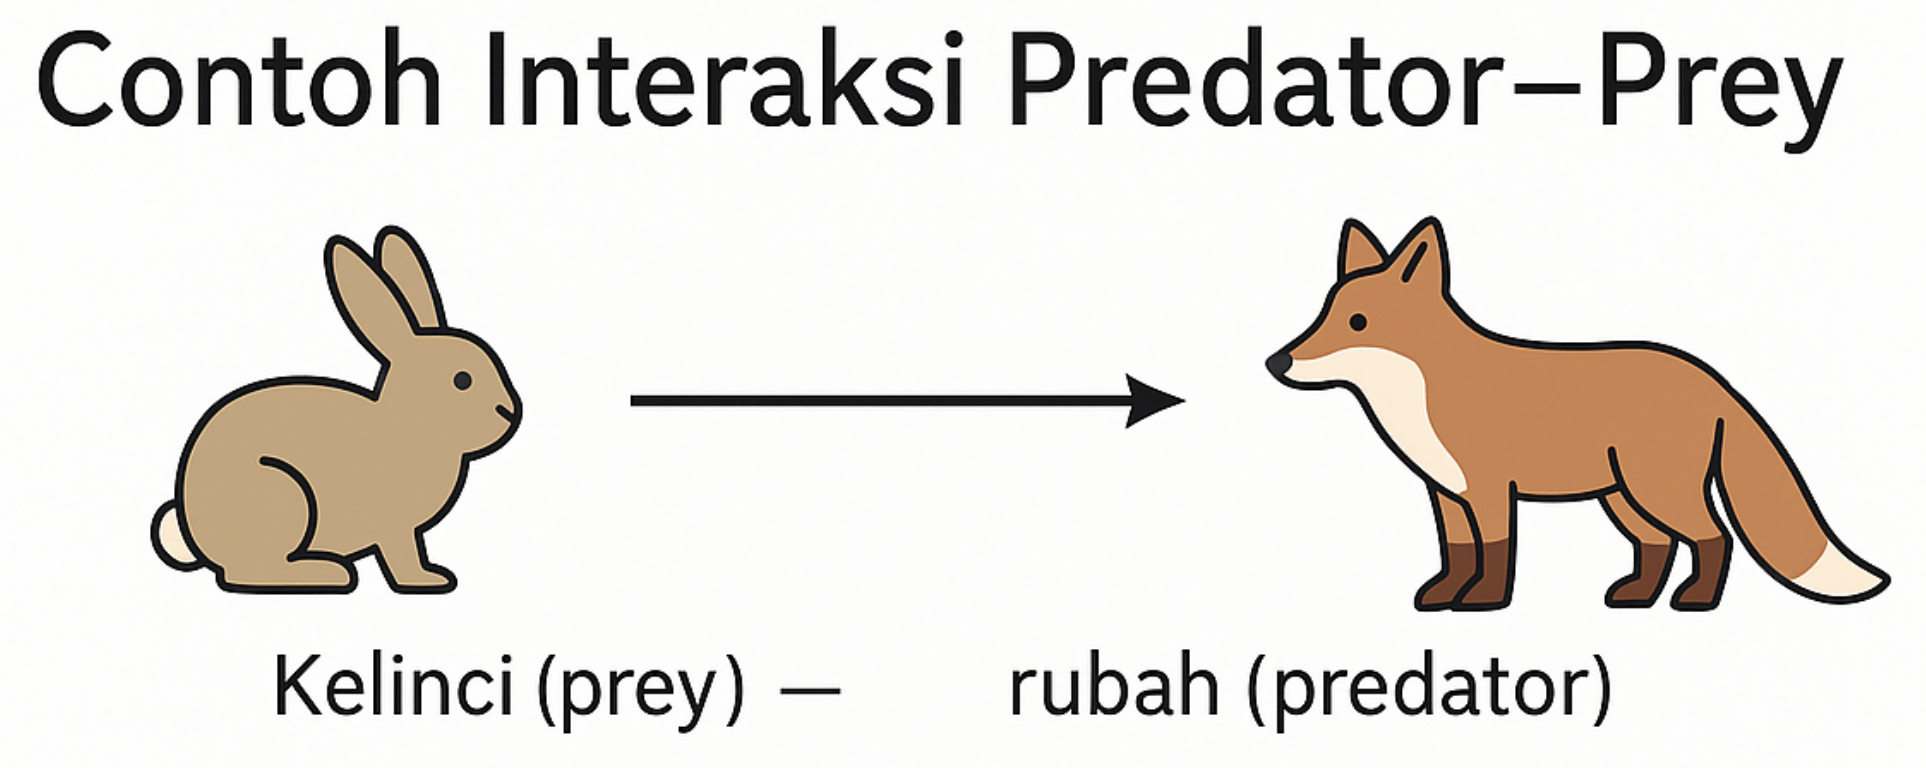
\includegraphics[width=\textwidth]{predator-prey.png}
		  \end{block}
	  \end{column}
  \end{columns}
\end{frame}

% ===========================================================
\section{Formulasi Model}
% ===========================================================

\begin{frame}{Variabel dan Asumsi Dasar}
  \begin{columns}[t]
  \begin{column}{0.45\textwidth}
    \begin{itemize}
      \item \(x(t)\): jumlah prey pada waktu \(t\)
      \item \(y(t)\): jumlah predator pada waktu \(t\)
    \end{itemize}
    \vspace{0.5em}
    Asumsi:
    \begin{enumerate}
      \item Tanpa predator: \(\dot{x}=ax\), \(a>0\)
      \item Tanpa prey: \(\dot{y}=-cy\), \(c>0\)
      \item Interaksi sebanding \(xy\): prey berkurang, predator bertambah
    \end{enumerate}
  \end{column}
  \begin{column}{0.5\textwidth}
    \begin{block}{Sistem Lotka–Volterra}
      \[
      \begin{cases}
      \dot{x} = ax - bxy,\\
      \dot{y} = -cy + dxy,
      \end{cases}\quad a,b,c,d>0.
      \]
    \end{block}
    \begin{block}{Makna Parameter}
    	\begin{itemize}
    		\item \(a\): pertumbuhan prey;
    		\item \(b\): tingkat dimangsa
    		\item \(c\): kematian predator;
    		\item \(d\): efisiensi konversi
    	\end{itemize}
      
    \end{block}
  \end{column}
  \end{columns}
\end{frame}

% ===========================================================
\section{Analisis Model}
% ===========================================================

\begin{frame}{Nullcline dan Titik Kesetimbangan}
  \begin{columns}
    \begin{column}{0.5\textwidth}
      Nullcline:
      \[
      \begin{aligned}
        \dot{x}=0 &\iff x=0 \;\text{atau}\; y=\tfrac{a}{b},\\
        \dot{y}=0 &\iff y=0 \;\text{atau}\; x=\tfrac{c}{d}.
      \end{aligned}
      \]
      Titik setimbang:
      \[
      E_1=(0,0),\qquad E_2=\Big(\tfrac{c}{d},\tfrac{a}{b}\Big).
      \]
      \vspace{0.5em}
      \begin{block}{Interpretasi}
              \(E_1\): kepunahan total (ekstrem).\\
              \(E_2\): koeksistensi pada level tetap.
            \end{block}
    \end{column}
    \begin{column}{0.4\textwidth}
      \begin{block}{}
      	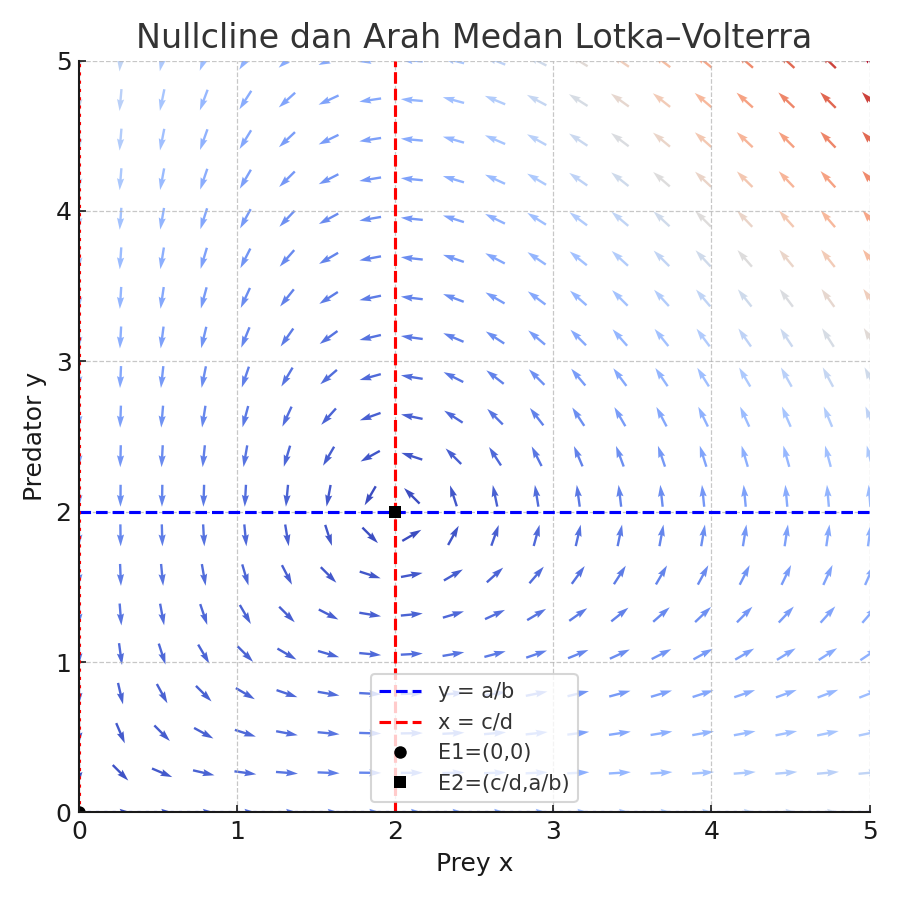
\includegraphics[width=\textwidth]{nullcline_field.png}
      \end{block}
      
    \end{column}
  \end{columns}
\end{frame}

\begin{frame}{Linearisation dan Jacobian}
  \small
  Sistem nonlinier: 
  \[
    \dot{x}=f(x,y), \quad \dot{y}=g(x,y).
  \]

  \textbf{Ide:} dekati sistem dengan bentuk linier di sekitar titik kesetimbangan.

  \vspace{0.5em}
  Matriks Jacobian:
  \[
    J(x,y) =
    \begin{pmatrix}
      \frac{\partial f}{\partial x} & \frac{\partial f}{\partial y} \\
      \frac{\partial g}{\partial x} & \frac{\partial g}{\partial y}
    \end{pmatrix}.
  \]

  \vspace{0.5em}
  Linearisation di sekitar $\mathbf{z}^*=(x^*,y^*)$:
  \[
    \dot{\Delta \mathbf{z}} \approx J(\mathbf{z}^*) \,\Delta \mathbf{z}, 
    \quad \Delta \mathbf{z}=\begin{pmatrix}x-x^*\\y-y^*\end{pmatrix}.
  \]

  \vspace{0.5em}
  \textbf{Eigenvalue $J(\mathbf{z}^*)$:}
  \begin{itemize}
    \item Re$(\lambda)<0$: stabil.
    \item Re$(\lambda)>0$: tak stabil.
    \item Im$(\lambda)\neq 0$: osilasi (spiral/center).
  \end{itemize}
\end{frame}

\begin{frame}{Aplikasi pada Lotka–Volterra}
  \small
  Sistem:
  \[
    \dot{x} = ax - bxy, \qquad 
    \dot{y} = -cy + dxy.
  \]

  Matriks Jacobian:
  \[
    J(x,y)=
    \begin{pmatrix}
      a - by & -bx \\
      dy & -c + dx
    \end{pmatrix}.
  \]

  \vspace{0.5em}
  Di $E_1=(0,0)$:
  \[
    J(E_1)=
    \begin{pmatrix} a & 0 \\ 0 & -c \end{pmatrix}
    \Rightarrow \lambda_1=a>0, \;\lambda_2=-c<0.
  \]
  $\Rightarrow$ \jsg{saddle tidak stabil}.

  \vspace{0.5em}
  Di $E_2=\big(\tfrac{c}{d},\tfrac{a}{b}\big)$:
  \[
    J(E_2)=
    \begin{pmatrix}
      0 & -\tfrac{bc}{d} \\
      \tfrac{da}{b} & 0
    \end{pmatrix}, \quad
    \operatorname{tr}=0,\;\det=ac>0.
  \]
  $\lambda_{1,2}=\pm i\sqrt{ac}$ $\;\Rightarrow\;$ \jsg{center (netral)}: orbit tertutup.
\end{frame}

\begin{frame}{Mencari Fungsi Invariant}
  \small
  Sistem Lotka–Volterra:
  \[
  \dot{x} = ax - bxy, \qquad \dot{y} = -cy + dxy.
  \]

  \vspace{0.5em}
  Tuliskan dalam bentuk rasio:
  \[
  \frac{\dot{x}}{x} = a - b y, 
  \qquad 
  \frac{\dot{y}}{y} = -c + d x.
  \]

  \vspace{0.5em}
  Ide: cari kombinasi yang merupakan turunan total suatu fungsi.
  Misal kandidat $H(x,y)$ dengan
  \[
    \pdv{H}{x} = d - \frac{c}{x}, 
    \qquad
    \pdv{H}{y} = b - \frac{a}{y}.
  \]

  \vspace{0.5em}
  Integrasi memberi:
  \[
    H(x,y) = d x - c \ln x + b y - a \ln y + \text{konst}.
  \]
\end{frame}

\begin{frame}{Invariant Pertama (Integral Konstan)}
  \small
  Fungsi konservasi:
  \[
  H(x,y)=d\,x- c\,\ln x + b\,y - a\,\ln y,\quad x>0,\;y>0.
  \]

  \vspace{0.5em}
  Verifikasi:
  \[
  \dot{H} = \pdv{H}{x}\dot{x} + \pdv{H}{y}\dot{y} = 0.
  \]

  \vspace{0.5em}
  \begin{block}{Konsekuensi}
    $H(x,y)$ tetap konstan sepanjang lintasan.\\
    Level set $H=\text{konst}$ adalah \textbf{orbit tertutup}.\\
    $\Rightarrow$ tidak ada atraktor/repellor dalam interior, hanya \textbf{osilasi netral}.
  \end{block}
\end{frame}

\begin{frame}{Invariant Pertama (Integral Konstan)}
  \small
  Sistem memiliki fungsi Lyapunov/konservasi:
  \[
  H(x,y)=d\,x- c\,\ln x + b\,y - a\,\ln y,\quad x>0,\;y>0,
  \]
  yang \textit{konstan} sepanjang solusi (level set \(H=\text{konst}\) adalah kurva orbit tertutup).
  \begin{block}{Konsekuensi}
    Tidak ada atraktor/repellor dalam interior: osilasi berkelanjutan (tanpa peredaman) \textit{di model dasar}.
  \end{block}
\end{frame}

\begin{frame}{Gambar Fase (Skema)}
  \centering
  \begin{tikzpicture}[scale=0.8]
    % axes
    \draw[-{Stealth[length=3mm]}] (0,0) -- (10,0) node[right]{$x$ (prey)};
    \draw[-{Stealth[length=3mm]}] (0,0) -- (0,6) node[above]{$y$ (predator)};
    % nullclines
    \draw[dashed] (7.0,0) -- (7.0,5.5) node[above] {$x=\tfrac{c}{d}$};
    \draw[dashed] (0,3.5) -- (9.5,3.5) node[right] {$y=\tfrac{a}{b}$};
    % equilibrium
    \filldraw (7.0,3.5) circle (2pt) node[above right] {$E_2$};
    % closed orbit
    \draw[very thick,blue] (7.0,3.5) ellipse [x radius=2.3, y radius=1.4];
    % orientation hint
    \draw[->,blue] (9.3,3.5) -- ++(0,0.25);
  \end{tikzpicture}
\end{frame}

% ===========================================================
\section{Sifat Dinamika}
% ===========================================================

\begin{frame}{Siklus Populasi (Narasi Kualitatif)}
  \begin{enumerate}
    \item Prey melimpah \(\Rightarrow\) predator bertambah.
    \item Predator naik \(\Rightarrow\) prey tertekan dan turun.
    \item Prey rendah \(\Rightarrow\) predator kekurangan makanan, turun.
    \item Predator turun \(\Rightarrow\) prey pulih. \(\Rightarrow\) ulang.
  \end{enumerate}
  \vspace{0.4em}
  \begin{block}{Catatan}
    Siklus periodik bersifat \jsg{netral} pada model dasar; di alam cenderung tidak sempurna karena faktor eksternal.
  \end{block}
\end{frame}

% ===========================================================
\section{Keterbatasan Model}
% ===========================================================

\begin{frame}{Mengapa Terlalu Sederhana?}
  \begin{itemize}
    \item Tidak ada \jsg{kapasitas lingkungan} untuk prey.
    \item Predator \jsg{tanpa kejenuhan} konsumsi (linear pada \(x\)).
    \item Abaikan \jsg{kompetisi intra-spesies} dan faktor lingkungan (musim, penyakit, migrasi, stokase).
    \item Hasil: \jsg{siklus sempurna} yang jarang terjadi di alam.
  \end{itemize}
\end{frame}

% ===========================================================
\section{Modifikasi Model}
% ===========================================================

\begin{frame}{Prey dengan Pertumbuhan Logistik}
  \begin{block}{Model}
  \[
  \dot{x}= ax\Big(1-\frac{x}{K}\Big) - bxy,\qquad
  \dot{y}= -cy + dxy.
  \]
  \end{block}
  \begin{itemize}
    \item \(K\): kapasitas lingkungan \(\Rightarrow\) mencegah pertumbuhan tak terbatas.
    \item Menstabilkan dinamika pada kondisi predator rendah.
  \end{itemize}
\end{frame}

\begin{frame}{Respon Fungsional Holling Tipe II}
  \begin{block}{Model}
  \[
  \dot{x}= ax - \frac{bxy}{1+h x},\qquad
  \dot{y}= -cy + \frac{dxy}{1+h x},\quad h>0.
  \]
  \end{block}
  \begin{itemize}
    \item \(h\): waktu penanganan (\textit{handling time}).
    \item Laju konsumsi predator \jsg{jenuh} saat prey melimpah.
  \end{itemize}
\end{frame}

\begin{frame}{Multi-Spesies (Dua Predator, Satu Prey)}
  \small
  \[
  \dot{x}= ax - b_1 x y_1 - b_2 x y_2,\quad
  \dot{y}_1= -c_1 y_1 + d_1 x y_1,\quad
  \dot{y}_2= -c_2 y_2 + d_2 x y_2.
  \]
  \begin{itemize}
    \item Dapat mengeksplor \jsg{kompetisi antar predator}.
    \item Memperluas analisis kestabilan dan kemungkinan bifurkasi.
  \end{itemize}
\end{frame}

% ===========================================================
\section{Latihan}
% ===========================================================

\begin{frame}{Latihan 1 — Titik Nol}
  Tunjukkan bahwa \(E_1=(0,0)\) tidak stabil.
  \begin{enumerate}
    \item Hitung \(J(E_1)\) dan eigenvalue-nya.
    \item Jelaskan makna ekologisnya (prey muncul sedikit \(\Rightarrow\) tumbuh; sistem menjauhi nol).
  \end{enumerate}
\end{frame}

\begin{frame}{Latihan 2 — Koeksistensi}
  Untuk \(a=1\), \(b=0.1\), \(c=1\), \(d=0.1\), hitung
  \[
  (x^\ast,y^\ast)=\Big(\tfrac{c}{d},\tfrac{a}{b}\Big)= (10,10).
  \]
  Apakah nilai ini masuk akal secara ekologis? Diskusikan.
\end{frame}

\begin{frame}[fragile]{Latihan 3 — Simulasi Komputasi}
  


\begin{columns}
	\begin{column}{0.35\textwidth}	
	Kondisi awal: \(x(0)=40\), \(y(0)=9\).
	  \begin{itemize}
	    \item Gambar \(x(t)\), \(y(t)\) terhadap waktu.
	    \item Plot lintasan fase \((x,y)\).
	  \end{itemize}
	\end{column}
	\begin{column}{0.625\textwidth}
		\begin{block}{Contoh Python (\texttt{solve\_ivp}):}
\begin{minted}{python}
import numpy as np
from scipy.integrate import solve_ivp
import matplotlib.pyplot as plt
a, b, c, d = 1.0, 0.1, 1.0, 0.1
def f(t, z):
    x, y = z
    return [a*x - b*x*y, -c*y + d*x*y]
sol = solve_ivp(f, [0, 100], [40, 9], dense_output=True)
T = np.linspace(0, 100, 2000)
X, Y = sol.sol(T)
plt.figure(); plt.plot(T, X); plt.plot(T, Y)
plt.figure(); plt.plot(X, Y)
plt.show()
\end{minted}
		\end{block}
	\end{column}
\end{columns}



\end{frame}

\begin{frame}{Latihan 4 — Refleksi Kritis}
  Mengapa model dasar sering dianggap terlalu sederhana? Pertimbangkan:
  \begin{itemize}
    \item Kapasitas lingkungan, kejenuhan predator.
    \item Musiman, penyakit, migrasi, stokastisitas.
    \item Data empiris: kapan model perlu dimodifikasi?
  \end{itemize}
\end{frame}

% ===========================================================
\section{Penutup}
% ===========================================================

\begin{frame}{Ringkasan}
  \begin{itemize}
    \item Model Lotka–Volterra: dua ODE dengan interaksi bilinear.
    \item Dua kesetimbangan: \(E_1\) (saddle), \(E_2\) (center netral).
    \item Orbit tertutup \(\Rightarrow\) siklus populasi; namun alam nyata lebih kompleks.
    \item Modifikasi: logistik prey, Holling II, multi-spesies.
  \end{itemize}
\end{frame}

\begin{frame}{Terima kasih!}
  \centering
  Pertanyaan?
\end{frame}

\begingroup
  \setbeamercolor{background canvas}{bg=black}
  \begin{frame}[plain]
    \centering
    % versi clean (tanpa margin, full black)
    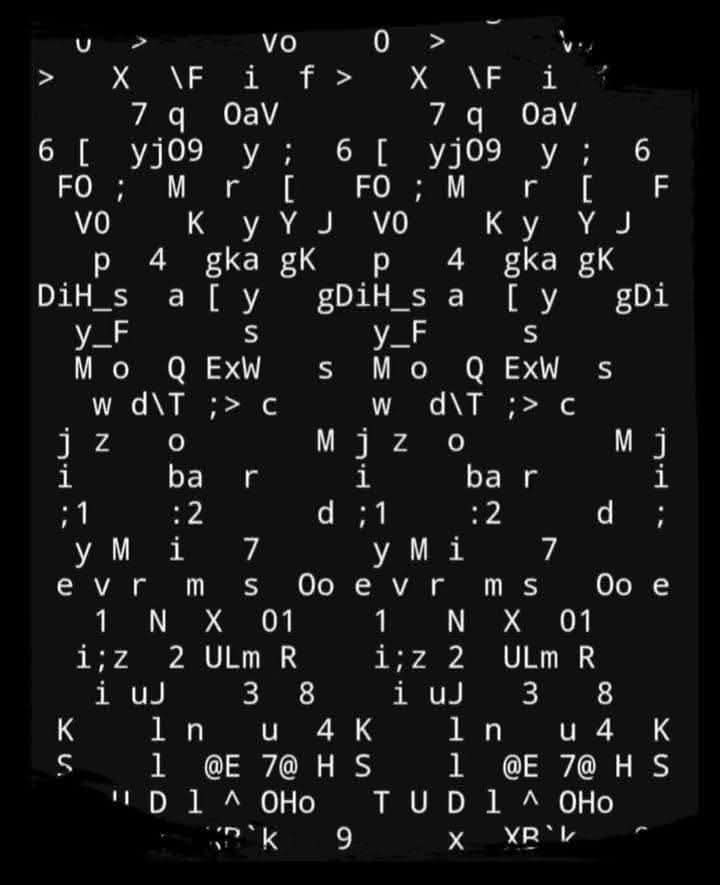
\includegraphics[height=.95\paperheight]{happy.jpg}
  \end{frame}
\endgroup

\appendix
\section{Lampiran}

\begin{frame}{Turunan Invariant \(H\)}
  \small
  \[\dot{H}=\pdv{H}{x}\dot{x}+\pdv{H}{y}\dot{y}\].
  
  Dengan 
  
  \[\pdv{H}{x}=d-\frac{c}{x}, \qquad \pdv{H}{y}=b-\frac{a}{y}\],
  
  dan 
  
  \[\dot{x}=ax-bxy, \qquad \dot{y}=-cy+dxy,\]
  
  diperoleh \(\dot{H}=0\).
\end{frame}

\begin{frame}{Catatan Teknis}
  \begin{itemize}
    \item Asumsi parameter \(a,b,c,d>0\); domain positif \(x,y>0\).
    \item Linearasi lokal valid dekat kesetimbangan; global: level set \(H\).
    \item Realisme: tambahkan faktor eksternal/derau untuk memecah degenerasi center.
  \end{itemize}
\end{frame}

\begin{frame}{Mencari Invariant $H(x,y)$}
  \small
  \textbf{Langkah 1.} Syarat konservasi:
  \[
    \dot{H}(x,y) \;=\; \pdv{H}{x}\dot{x} + \pdv{H}{y}\dot{y} \;=\; 0.
  \]

  Sistem Lotka–Volterra:
  \[
    \dot{x} = ax - bxy, \qquad \dot{y} = -cy + dxy.
  \]

  \vspace{0.5em}
  \textbf{Langkah 2.} Tebak bentuk turunan parsial agar saling meniadakan:
  \[
    \pdv{H}{x} = d - \frac{c}{x}, 
    \qquad 
    \pdv{H}{y} = b - \frac{a}{y}.
  \]

  \vspace{0.5em}
  Dengan pilihan ini, setiap suku pada $\dot{H}$ dari $\dot{x}$ dan $\dot{y}$ saling membatalkan.
\end{frame}

\begin{frame}{Hasil Invariant Pertama}
  \small
  \textbf{Langkah 3.} Integrasi turunan parsial:
  \[
    H(x,y) = d\,x - c \ln x + b\,y - a \ln y + \text{konst}.
  \]

  \vspace{0.5em}
  Verifikasi:
  \[
    \dot{H} = \pdv{H}{x}\dot{x} + \pdv{H}{y}\dot{y} = 0.
  \]

  \vspace{0.5em}
  \begin{block}{Konsekuensi}
    $H(x,y)$ tetap konstan sepanjang lintasan.\\
    Level set $H=\text{konst}$ adalah \textbf{orbit tertutup}.\\
    $\Rightarrow$ osilasi netral tanpa peredaman pada model dasar.
  \end{block}
\end{frame}

\begin{frame}{Dari mana $H(x,y)$ berasal? (tanpa tebak)}
  \small
  \textbf{Eliminasi $t$:}
  \[
    \frac{dy}{dx}=\frac{-cy+dxy}{ax-bxy}
    =\frac{y(-c+dx)}{x(a-by)}.
  \]
  Kalikan silang:
  \[
    \frac{a-by}{y}\,dy+\frac{-c+dx}{x}\,dx=0
    \;\Longleftrightarrow\;
    \bigl(d-\tfrac{c}{x}\bigr)dx+\bigl(b-\tfrac{a}{y}\bigr)dy=0.
  \]
  Bentuk ini \textbf{eksak}: ada $H$ dengan
  \[
    dH=(d-\tfrac{c}{x})\,dx+(b-\tfrac{a}{y})\,dy.
  \]
  Integrasi memberi
  \[
    \boxed{H(x,y)=d\,x-c\ln x+b\,y-a\ln y}.
  \]
  Sepanjang solusi: $\dot H=0$ $\Rightarrow$ $H$ konstan (level set = orbit).
\end{frame}

\begin{frame}{Asal-usul Respon Fungsional Holling Tipe II}
  \small
  \textbf{Latar belakang:} Predator tidak bisa makan tanpa batas.
  Ada waktu untuk menangkap dan mencerna mangsa 
  $\Rightarrow$ laju konsumsi \textbf{jenuh}.

  \vspace{0.5em}
  \textbf{Formulasi Holling (1959):}
  \[
    \text{Consumption per predator} 
    = \frac{\alpha x}{1+\alpha h x},
  \]
  dengan:
  \begin{itemize}
    \item $\alpha$: laju serangan (attack rate),
    \item $h$: \jsg{handling time} (waktu penanganan per mangsa).
  \end{itemize}

  \vspace{0.5em}
  \textbf{Sifat:}
  \begin{itemize}
    \item Jika $x$ kecil: $\;\frac{\alpha x}{1+\alpha h x} \approx \alpha x$
      $\;\Rightarrow$ mirip Lotka–Volterra.
    \item Jika $x \to \infty$: $\;\frac{\alpha x}{1+\alpha h x} \to \tfrac{1}{h}$
      $\;\Rightarrow$ jenuh (konstan).
  \end{itemize}
\end{frame}

\begin{frame}{Ilustrasi Kurva Jenuh Holling II}
  \centering
  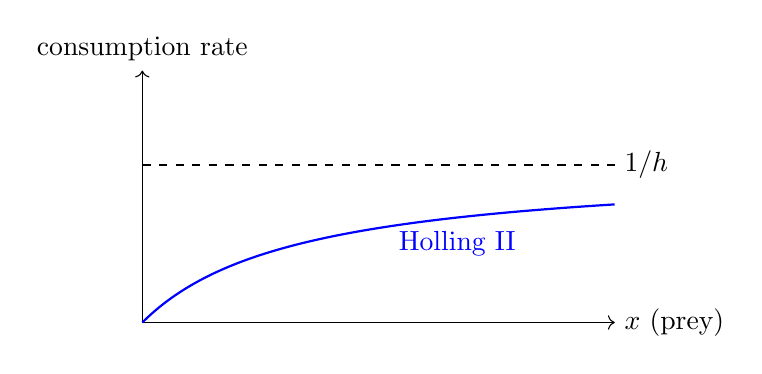
\begin{tikzpicture}[scale=1.0]
    \draw[->] (0,0) -- (6,0) node[right] {$x$ (prey)};
    \draw[->] (0,0) -- (0,3.2) node[above] {consumption rate};
    % curve: alpha=1, h=0.5
    \draw[thick,blue,domain=0:6,samples=100] 
      plot(\x,{(1*\x)/(1+0.5*\x)});
    % dashed horizontal asymptote
    \draw[dashed] (0,2) -- (6,2) node[right] {$1/h$};
    \node at (4,1) [blue] {Holling II};
  \end{tikzpicture}

  \vspace{0.5em}
  \textit{Kurva konsumsi jenuh: awalnya linear, lalu mendekati asimtot $1/h$.}
\end{frame}

\begin{frame}{Limit pada Model Holling II yang Kita Pakai}
  \small
  \[
    \dot{x}= ax - \frac{bxy}{1+h x},\qquad
    \dot{y}= -cy + \frac{dxy}{1+h x},\quad h>0.
  \]
  \vspace{0.4em}
  \textbf{Prey sedikit ($x\to 0$):} 
  \(\;\frac{bxy}{1+hx}\approx bxy,\;\frac{dxy}{1+hx}\approx dxy\)
  \(\Rightarrow\) kembali ke Lotka–Volterra (linier pada $x$).
  \vspace{0.3em}

  \textbf{Prey melimpah ($x\to\infty$):} 
  \(\;\frac{bxy}{1+hx}\approx \frac{b}{h}y,\;
    \frac{dxy}{1+hx}\approx \frac{d}{h}y\)
  \(\Rightarrow\) laju predasi dan pertumbuhan predator \textbf{jenuh} (tak naik lagi dengan $x$).
  \vspace{0.4em}

  \begin{block}{Makna Parameter}
    $b$: laju serangan efektif; \quad
    $h$: handling time; \quad
    $d$: efisiensi konversi. \\
    Kapasitas maksimum konsumsi per predator $\sim b/h$, 
    dan maksimum pertumbuhan karena makan $\sim d/h$.
  \end{block}
\end{frame}

\end{document}
